\chapter{Introduction}
\textit{Static analysis} is a widely used technique for finding \textit{vulnerabilities} during software development. \textit{Static analyzers} can also be deployed on code that is not yet finished. This makes it possible to detect vulnerabilities in the early stages of development, even before tests can be run. However, static analyzers often suffer from a high number of \textit{false positives}. If the percentage of false positives is too high, these tools are almost unusable in practice. Therefore, a lot of effort is devoted to the automatic detection of false positives.

This thesis focuses on the Meta Infer static analyzer. It is a highly \textit{scalable}, \textit{interprocedural}, \textit{open-source} tool for analyzing C/C++/C\#/Obj-C and Java source files. Compared to other static analyzers, it is characterized by its ease of use -- its input is compilation commands that compile the analyzed source files. Although it is a very useful tool, it does have its disadvantages and the main one is the high number of false positives. From experiments conducted in the author's Bachelor's thesis, it was found that up to almost 90~\% of the reports are false positives.

The main contribution of the future Master's thesis is the design and implementation of a \textit{false positive detection system} for the Meta Infer tool. If reports that are likely to be false positives could be detected and subsequently removed, it would be possible to reduce the amount of false positives that Infer produces. Thus, the proposed detection system could make Infer a more practical tool because the current percentage of false positives is too high. The input to the detection system is the source files and list of vulnerabilities from Infer. The output will then be, for each vulnerability found by Infer, the probability that it is a false positive. The detection system is based on \textit{graph neural networks} (GNN), which have proven to be very powerful tool for finding vulnerabilities in source code. The detection system is composed of two parts -- the graph construction and the GNN detection model. 

The main contribution of this term project is the design of the first part of the false positive detection system -- the construction of graphs from source code. This part is designed as a pipeline that connects to the running \textit{compilation} process of the analyzed software and constructs graphs from the compiled source files. The output of this pipeline is \textit{code property graphs} (CPG) -- a very widely used graphical representation of code for vulnerability detection that captures the \textit{syntactic} and \textit{semantic} properties of the code. The pipeline internally uses the LLVM intermediate representation (LLVM IR), from which it then constructs, for each vulnerability found by Infer, a single CPG that represents the vulnerability. The use of LLVM IR makes the output graph independent of the pipeline input language. And since the vulnerability found by Infer is only used in the pipeline to extract criteria for the \textit{program slicing}, the resulting graph is also independent of the used static analyzer.


\paragraph{Acknowledgement.} This term project is in collaboration with Red Hat. It is also supported by projects H2020 ECSEL Valu3s, GACR AIDE 23-06506S, and IGA FIT-S-23-8151.

\paragraph{Structure of the term project.}
 The rest of this term project is structured as follows. Chapter \ref{preliminaries} explains basic principles of static analysis and graph neural networks. The chapter also describes code property graphs and tools used in this term project, namely Meta Infer, LLVM-Slicer, LLVM2CPG and Joern. Chapter \ref{pipeline} describes the design of a~pipeline for automatic extraction of code property graphs from source files. Chapter \ref{future-work} describes future work, specifically \textit{automation} of the proposed pipeline, transformation of the D2A dataset to code property graphs, selection of a graph neural network architecture, \textit{self-training} technique, integration with the csmock tool, and the data for the experiments. This term project together with the future work presented in Chapter \ref{future-work} will form the Master's thesis.


\chapter{Preliminaries}
\label{preliminaries}
This chapter introduces the basic concepts, principles and tools on which this term project builds. Specifically, Section \ref{static-analysis} briefly describes static analysis itself, its applications, advantages and limitations. Section \ref{infer} describes the Meta Infer static analyzer, its use, types of \textit{detectable vulnerabilities}, and its advantages and disadvantages. Section \ref{gnn} describes the general principle of graph neural networks, their advantages for source code analysis, and especially their input format. Section \ref{cpg} introduces the different \textit{source code representations} used as input to graph neural networks and focuses on the most commonly used type - code property graphs. Section \ref{slicer} presents the LLVM- Slicer for \textit{slicing} LLVM bitcode. Section \ref{llvm2cpg} describes a tool for constructing code property graphs from LLVM bitcode. Finally, Section \ref{joern} presents the Joern platform used for various static analysis tasks.

\section{Static Analysis}
\label{static-analysis}

Static analysis \cite{bc, static-analysis-EMANUELSSON20085, testovani-herout} can be understood as a \textit{reasoning} of \textit{run-time properties} of computer programs without the need to run them or provide their inputs. Using static analysis, it is possible to investigate program properties such as \textit{time} or \textit{memory complexity}, look for \textit{security risks} such as \textit{null pointer dereference}, \textit{access beyond array boundaries}, improper handling of resources, etc. It is also possible to check for \textit{synchronization errors} such as \textit{deadlock}, \textit{data race}, \textit{atomicity violation}, etc. Finally, static analysis can be used to ensure compliance with language standards e.g. MISRA-C/MISRA-C++\footnote{\textbf{MISRA}'s website: \url{https://www.misra.org.uk/}.} or compliance with practices for writing readable code e.g. Google Java Style\footnote{\textbf{Google Java Style Guide}: \url{https://google.github.io/styleguide/javaguide.html}.}.

The opposite of static analysis is \textit{dynamic analysis}, which requires running the program to be analyzed and thus inserting possible inputs. Since both approaches have their advantages and disadvantages, it is not advisable to use only one, but rather to use both simultaneously to complement each other. The advantages of static analysis are \cite{bc, static-analysis-pros-cons}:
\begin{itemize}
    \item implicitly consider all possible paths in the code (even the ones with rare execution path),
    \item can report the exact location of the vulnerability and thus speed up the fix,
    \item do not require executable, sometimes even compilable source code, so bugs can be detected early in development,
    \item after the initial setup, they can be run fully automatically.
\end{itemize}

However, static analysis also has its disadvantages \cite{testovani-herout, static-analysis-pros-cons}:
\begin{itemize}
    \item static analyzers usually do not have information about \textit{functional requirements} and thus cannot be used for \textit{validation},
    \item initial setup can be tedious for some tools, as it may require e.g. creating \textit{models} of certain functions, accessing compilation of a code, or manually editing the required style guide,
    \item static analysis also cannot be used to check the \textit{semantic function} of a program (e.g. does the program give the correct result?),
    \item running static analyzers can be very time and memory consuming,
    \item static analyzers can report false positives (false reports) or \textit{false negatives} (missed real errors).
\end{itemize}

\textit{Rice's theorem} implies \cite{static-analysis-spa} that all non-trivial properties of program behavior are \textit{undecidable}. From this it follows that in order to derive such properties automatically, it is necessary to introduce some degree of \textit{approximation}. This approximation is the cause of false positives and false negatives. However, if a suitable approximation is used, it is possible to use static analysis to prove some properties (as opposed to dynamic analysis) - typically the absence of errors. An example of this behavior is the use of Frama-C to create an RTE- free\footnote{\textbf{Run Time Error (RTE)}.} X.509 parser \cite{RTEFreeParser}. However, most tools try to create approximations that balance the number of false positives and false negatives to make the tools practical to use.

\section{Meta Infer}
\label{infer}
Meta Infer \cite{infer-web} (formerly Facebook Infer) is an open-source\footnote{\textbf{Meta Infer}'s repository: \url{https://github.com/facebook/infer/}.} \textit{framework} for writing \textit{intraprocedural} and \textit{interprocedural} static analyses \cite{harmim-dip, marcin-bc, marek-bc}. Although it is a framework, Infer already includes a number of default and non-default (they must be explicitly enabled) analyses. Individual analyses are plugged into Infer in the form of \textit{plugins}. Different plugins use different principles to detect different types of vulnerabilities, e.g. InferBO, which uses the \textit{symbolic interval} technique \cite{InferBO} to detect incorrect array indexing, or the Bi-abduction plugin, which uses \textit{bi-abduction} \cite{SeparationLogic} -- a form of \textit{inference} for \textit{separation logic} that models computer memory -- to detect vulnerabilities associated with incorrect memory manipulation. Among other things, Infer can detect \textit{null-pointer dereference}, \textit{dead store}, \textit{uninitialized value}, \textit{deadlock}, \textit{data race}, \textit{variable overflow}, and many other types of vulnerabilities. Table~\ref{table:infer-plugins} lists all the plugins that Infer provides, along with information about language support and whether the plugin is enabled by default. More detailed information about each plugin and the types of vulnerabilities reported by Infer can be found at \cite{AllIssues}.

\begin{table}
\centering
\caption{Language support information for all non-experimental Infer plugins, along with
whether the plugins are enabled by default.}
\label{table:infer-plugins}
\begin{tabular}{ !{\vrule width 1pt}l!{\vrule width 1pt}c|c|c|c|c!{\vrule width 1pt}c!{\vrule width 1pt} } 
 \noalign{\hrule height 1pt}
 \hspace{1.65cm}\textbf{Plugin} & \textbf{C} & \textbf{C++} & \textbf{Objective C} & \textbf{Java} & \textbf{C\#} & \textbf{Default} \\ 
 \noalign{\hrule height 1pt}
 Annotation Reachability & \checkmark & \checkmark & \checkmark & \checkmark & \checkmark &  \\ 
 \hline
 Bi-abduction & \checkmark & \checkmark & \checkmark & \checkmark & \checkmark & \checkmark \\ 
 \hline
 InferBO & \checkmark & \checkmark & \checkmark & \checkmark & \checkmark &  \\ 
 \hline
 Cost & \checkmark & \checkmark & \checkmark & \checkmark & \checkmark &  \\ 
 \hline
 Eradicate &  &  &  & \checkmark & \checkmark &  \\ 
 \hline
 Impurity & \checkmark & \checkmark & \checkmark & \checkmark & \checkmark &  \\ 
 \hline
 Inefficient keySet Iterator &  &  &  & \checkmark & \checkmark & \checkmark \\ 
 \hline
 Litho "Required Props" &  &  &  & \checkmark & \checkmark &  \\ 
 \hline
 Liveness & \checkmark & \checkmark & \checkmark &  &  & \checkmark \\ 
 \hline
 Loop Hoisting & \checkmark & \checkmark & \checkmark & \checkmark & \checkmark &  \\ 
 \hline
 Pulse & \checkmark & \checkmark & \checkmark & \checkmark &  &  \\ 
 \hline
 Purity & \checkmark & \checkmark & \checkmark & \checkmark & \checkmark &  \\ 
 \hline
 Quandary & \checkmark & \checkmark & \checkmark & \checkmark & \checkmark &  \\ 
 \hline
 RacerD &  & \checkmark &  & \checkmark & \checkmark & \checkmark \\ 
 \hline
 .NET Resource Leak &  &  &  &  & \checkmark & \checkmark \\ 
 \hline
 SIOF &  & \checkmark &  &  &  & \checkmark \\ 
 \hline
 Self in Block &  & \checkmark & \checkmark &  &  & \checkmark \\ 
 \hline
 Starvation & \checkmark & \checkmark & \checkmark & \checkmark & \checkmark & \checkmark \\ 
 \hline
 Uninit & \checkmark & \checkmark & \checkmark &  &  & \checkmark \\ 
 \noalign{\hrule height 1pt}
\end{tabular}
\end{table}

Infer is not a \textit{sound}, which in the context of finding vulnerabilities means that it may miss some (it may have a false negatives). Instead, it aims for maximal practical use - scaling to millions of lines of code thanks to \textit{modular analysis}. It is also very simple to use \cite{infer-usage} compared to other analyzers. Infer takes as an input compilation commands that allow the Infer's internal clang compiler to transform source files into the SIL\footnote{\textbf{Smallfoot Intermediate Language (SIL)}.} internal representation~\cite{SIL2, SIL}. This transformation (\textit{capture}) of the source code takes place in the capture phase. To facilitate the capture of compilation commands, Infer supports a~variety of \textit{build systems} such as ant, cmake, Gradle, Make, Maven, and others. However, experiments conducted in previous work by the author \cite{bc} show that this support is not complete and often fails to capture compilation commands. Therefore, as part of the same work, a compiler wrapper was created that can reliably capture compilation commands and pass them to Infer.

The capture phase is followed by an analysis phase in which the required plugins are run over the SIL. The output of Infer after the analysis phase is a list of found vulnerabilities. Experiments on \textit{real-world} programs in previous work \cite{bc} also show that Infer has a very high number of false positives. Specific numbers suggest approximately 4.5 false positives for every real vulnerability. However, this score is very optimistic since it includes dead store errors, which are harmless and can be detected by common compilers and are present in real-world programs in very large numbers - especially in C language while using conditional compilation. Without dead stores the number increases to approximately 9 false positives for every real vulnerability. The high number of false positives in static analyzers results in developers' distrust of these tools and consequent ignoring of analysis results~\cite{InferInFB, DisadvantagesOfStaticAnalysis, DisadvantagesOfStaticAnalysis2}. Therefore, efforts are made to reduce false positives.

\section{Graph Neural Networks}
\label{gnn}

There are a number of approaches for detecting vulnerabilities in programs using \textit{machine learning} \cite{taxonomy-hanif2021rise}. However, when focusing on the area of \textit{deep learning}, approaches can be divided into \textit{convolutional neural networks} (CNN) \cite{CNN1-MIX-duan2019vulsniper}, \textit{recurrent neural networks} (RNN)~\cite{RNN5-li2021vuldeelocator, RNN2-li2021sysevr, RNN3-li2018vuldeepecker, RNN6-lin2017poster, RNN7-saccente2019project, RNN4-zou2019mu} and graph neural networks (GNN)~\cite{GNN1-cao2021bgnn4vd, GNN3-cheng2021deepwukong, GNN6-ganz2021explaining, GNN5-vsikic2022graph, GNN4-IBM-suneja2020learning, GNN2-zhou2019devign}, depending on the \textit{architecture} of the model used. These approaches are often combined with each other~\cite{GNN8-RNN-fang2022jstrong, CNN1-RNN-li2020automated, GNN7-RNN-rabheru2020hybrid, RNN1-CNN-russell2018automated}.

CNNs achieve very good results, e.g. in \textit{image classification}. This is aided by \textit{convolutional layers} that can appropriately capture \textit{spatial information} from an image. However, this principle is not so effective for source code \cite{gnn-usage}. In order to use the source code as input to a CNN, it must first be transformed into a graph (e.g. AST) and then into a matrix (e.g. \textit{adjacency matrix}). Due to the fact that the nodes in a graph do not have a fixed order, the same graph can be expressed as a adjacency matrix (which has a fixed order of nodes) in multiple ways. This property is very undesirable because we want the same result for the same graph. It also makes it impossible to use the \textit{local spatial properties} of convolutional layers. Another problem for CNN is the arbitrary size of the graph.

Another frequently used approach is to represent code as a \textit{sequence}, especially for recurrent neural networks. This approach is based on the idea that the source code can be treated as a \textit{natural language}. While these approaches achieve very good results \cite{NLP-APPROACH1-buratti2020exploring, NLP-APPROACH2-hanif2022vulberta}, the properties of source code can be better represented using graphs. Appropriately designed graphs can more explicitly model properties between parts of the code that would otherwise the model had to learn during training. The idea that a graph is a better representation of source code than a picture or a sequence is supported by the experiments in \cite{GNN4-IBM-suneja2020learning}, especially on \textit{synthetic datasets} (on \textit{datasets} with real-world examples, all approaches failed in a given experiment).

For this term project, the most important thing is to define the format of the input graph. To make it clear what the format is based on, a brief description of a general graph neural network follows. The following description uses a slightly modified notation from \cite{GGNN-li2015gated}. 

Consider an \textit{oriented graph} structure $\mathcal{G} = (\mathcal{V}, \mathcal{E})$, where $\mathcal{V}$ is the \textit{set} of \textit{nodes} and $\mathcal{E}$ is the set of \textit{oriented edges} $\mathit{e} = ( \mathit{v}, \mathit{v}' ) \in \mathcal{V} \bigtimes \mathcal{V}$. The output node of edge $\mathit{e} = ( \mathit{v}, \mathit{v}' )$ is $\mathit{v}$ and the input node is $\mathit{v}'$. The \textit{embedding vector} of node $\mathit{v}$ is denoted by $\textbf{h}_\mathit{v} \in \mathbb{R}^\mathit{D}$, where $\mathit{D}$ is the \textit{dimension} of the vector. Each node has a \textit{label} which is denoted by $\mathit{l}_\mathit{v} \in \{1, ... , \mathit{L}_\mathcal{V}\}$ and each edge has a label which is denoted by $\mathit{l}_\mathit{e} \in \{1, ... , \mathit{L}_\mathcal{E}\}$. Further, we define auxiliary sets of nodes. The set $\textsc{In}(\mathit{v}) = \{\mathit{v}' | (\mathit{v}', \mathit{v}) \in \mathcal{E}\}$ contains the \textit{predecessors} of node $\mathit{v}$. The set $\textsc{Out}(\mathit{v}) = \{\mathit{v}' | (\mathit{v}, \mathit{v}') \in \mathcal{E}\}$ contains the \textit{descendants} of node $\mathit{v}$. \textit{Propagation} then proceeds by updating each node until \textit{convergence} using the following formula:

\begin{equation*}
	\textbf{h}_\mathit{v}^{(\mathit{t})} = \sum_{\mathit{v}' \in \textsc{In}(\mathit{v})} \mathit{f}(\mathit{l}_\mathit{v}, \mathit{l}_{(\mathit{v}', \mathit{v})}, \mathit{l}_{\mathit{v}'}, \textbf{h}_{\mathit{v}'}^{(\mathit{t}-1)}) + \sum_{\mathit{v}' \in \textsc{Out}(\mathit{v})} \mathit{f}(\mathit{l}_\mathit{v}, \mathit{l}_{(\mathit{v}, \mathit{v}')}, \mathit{l}_{\mathit{v}'}, \textbf{h}_{\mathit{v}'}^{(\mathit{t}-1)})
\end{equation*}

Where the function $\mathit{f}$ can be a \textit{linear function} $\textbf{h}_{\mathit{v}'}^{(\mathit{t})}$ or a \textit{neural network}. The output of this
network is for each node defined as $\mathit{o}_\mathit{v} = \mathit{g}(\textbf{h}_\mathit{v}^{(\mathit{T})}, \mathit{l}_\mathit{v})$, where $\mathit{g}$ is an arbitrary \textit{differentiable} function and $\mathit{T}$ is the final iteration. In case where \textit{graph-level classification}/\textit{regression} is needed, it is possible to artificially add a so-called "\textit{super node}" to the original graph, which will be connected to all nodes. This will allow graph-level classification/regression to be treated in the same way as \textit{node-level classification}/\textit{regression}.

The \textit{Almedia-Pineda algorithm} is used to learn such a model. Firstly, the algorithm runs the model until the values of $\textbf{h}_\mathit{v}^{(\mathit{T})}$ converge. These values must be \textit{constrained} to guarantee convergence. Since the whole GNN is differentiable, it is then possible to compute \textit{gradients} for parameter adjustments from the converged solution.

\section{Source Code as a Graph}
\label{cpg}

There are many types of graphs that are used as source code representations, e.g. \textit{abstract syntax trees} (AST), \textit{control flow graphs} (CFG), \textit{program dependency graphs} (PDG) and others. A very common type is the code property graph (CPG), which is composed of all three previous graphs and used in its pure form in e.g. \cite{USE-CPG-liu2020retrieval, GNN4-IBM-suneja2020learning}. Modified versions of it are often used as well, e.g. \textit{simplified CPGs} (SCPG) for \textit{function-level vulnerability detection} in C/C++ \cite{SCPG-wu2021vulnerability}, CPGs with added edges that reflect the original order of \textit{tokens} (individual source code elements) \cite{GNN2-zhou2019devign} or \textit{code composite graphs} (CCG) again for vulnerability detection in C/C++ \cite{GNN1-cao2021bgnn4vd}. Furthermore, e.g. PDGs alone are used for finding \textit{malicious code} in JavaScript \cite{GNN8-RNN-fang2022jstrong}, XFGs (\textit{subgraph} of PDG) for detecting vulnerabilities in C/C++ code \cite{GNN3-cheng2021deepwukong} or CFGs together with token sequences for detecting vulnerabilities in PHP~\cite{PHP-rabheru2020hybrid}.

According to \cite{CPG-yamaguchi2014modeling}, the reason for the creation of CPGs is the inability of each subgraph type to detect certain types of vulnerabilities independently during \textit{traversal}. For example, AST is not suitable for detecting \textit{division by zero}. However, by combining AST and PDG it is possible, but still cannot detect e.g. integer overflow. This can only be detected by combining AST, CFG and PDG. This combination of graphs results in a representation that is able to capture both syntactic and semantic properties of the code and preserve most types of vulnerabilities in it. Exceptions are e.g. \textit{race conditions}, which need more external information. A complete table is given in \cite{CPG-yamaguchi2014modeling}. The following graph definitions are based on the original definitions from the paper introducing CPGs \cite{CPG-yamaguchi2014modeling}, with only minor changes in notation (to resemble the GNN definition given earlier) and changes in some notations to make them formally correct.

To formally define a CPG, it is first necessary to define a \textit{property graph} \cite{CPG-yamaguchi2014modeling}, which is a~commonly used graph type in \textit{graph databases} such as Neo4j. Formally, a property graph is an oriented \textit{multigraph}  $\mathcal{G} = (\mathcal{V}, \mathcal{E}, \lambda, \mu)$, here $\mathcal{V}$ denotes the set of nodes, $\mathcal{E}$ denotes the set of edges, $\lambda$ denotes the \textit{edge labeling function} $\lambda : \mathcal{E} \rightarrow \Sigma$, where $\Sigma = {1, ..., L_\mathcal{E}}$ are the edge labels. Finally, $\mu$ denotes the function that assigns attributes to nodes and edges $\mu: (\mathcal{V} \cup \mathcal{E}) \bigtimes K \rightarrow S$, where $K$ is the set of \textit{attribute} names and $S$ is the set of attribute values.

\begin{lstlisting}[
    style=c++, label={listing:cpg}, float=hbt,
    caption={Code sample. The code was taken from~\cite{CPG-yamaguchi2014modeling}.}
]
void foo()
{
    int x = source();
    if (x < MAX)
    {
        int y = 2 * x;
        sink(y);
    }
}
\end{lstlisting}

\begin{figure}[hbt]
	\centering
	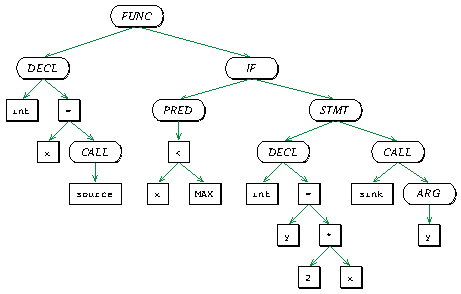
\includegraphics[width=0.75\textwidth]{figures/AST.pdf}
	\caption{Abstract syntax tree for the code in Listing \ref{listing:cpg}. This figure was taken from~\cite{CPG-yamaguchi2014modeling}.}
	\label{figure:AST}
\end{figure}

An AST \cite{CPG-yamaguchi2014modeling} is an \textit{ordered tree} whose inner nodes represent \textit{operators} and outer nodes (\textit{leaves}) represent \textit{operands}. The oriented edges then show the parenting relation. The AST captures the syntactic nature of the code. Consider the code in Listing \ref{listing:cpg}. An AST constructed for this code is shown in Figure \ref{figure:AST}. To create a formal CPG description, the subgraph types must be converted to the same format - the previously defined property graph. An AST as a property graph is a structure $\mathcal{G}_{\textsc{Ast}} = (\mathcal{V}_{\textsc{Ast}}, \mathcal{E}_{\textsc{Ast}}, \lambda_{\textsc{Ast}}, \mu_{\textsc{Ast}})$, where $\mathcal{V}_{\textsc{Ast}}$ is the set of AST nodes and $\mathcal{E}_{\textsc{Ast}}$ is the set of AST edges. The function $\lambda_{\textsc{Ast}}$ is defined as $\lambda_{\textsc{Ast}}(\mathit{v}) = \textrm'\textsc{Ast}\textrm'$ and is applied to each node $\mathit{v} \in \mathcal{V}_{\textsc{Ast}}$. The function~$\mu_{\textsc{Ast}}:~\mathcal{V_{\textsc{Ast}}}~\bigtimes~K_{\textsc{Ast}}~\rightarrow~S_{\textsc{Ast}}$ is applied to each node and attribute. The attribute names are $K_{\textsc{Ast}}~=~\{\textrm'code\textrm',~\textrm'order\textrm'\}$ and the attribute values are $S_{\textsc{Ast}}~=~S_{code}~\cup~S_{order}$, where $S_{code}$ are types of nodes in AST e.g. \textit{variable}, \textit{constant}, mathematical operators etc. And $S_{order}$ which assigns values (order) to nodes in the AST to preserve the ordering from the original tree.

\begin{figure*}[h]\centering
  \centering
  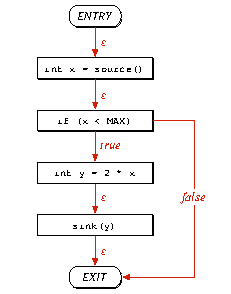
\includegraphics[width=0.36\linewidth]{figures/CFG.pdf}\hfill
  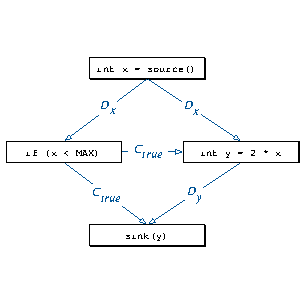
\includegraphics[width=0.48\linewidth]{figures/PDG.pdf}
  \caption{Control flow graph (on the left) and program dependence graph (on the right) for the code in Listing \ref{listing:cpg}. These figures were taken from~\cite{CPG-yamaguchi2014modeling}.}
  \label{figure:CFG-PDG}
\end{figure*}

A CFG \cite{CPG-yamaguchi2014modeling} is an oriented graph describing the possible paths of \textit{program control} and the conditions for their \textit{execution}. The nodes of the graph represent \textit{statements} and \textit{predicates}, while the edges represent \textit{control passing}. Each command node has an outgoing edge labeled~$\epsilon$, which denotes an \textit{unconditional} passing of control. While a predicate node must have two outgoing edges $true$ and $false$ for different evaluations of a given predicate. Consider the code in Listing \ref{listing:cpg}. A CFG constructed for this code is shown in Figure \ref{figure:CFG-PDG}. The CFG as a property graph is the structure $\mathcal{G}_{\textsc{Cfg}} = ( \mathcal{V}_{\textsc{Cfg}}, \mathcal{E}_{\textsc{Cfg}}, \lambda_{\textsc{Cfg}}, \cdot )$, where $\mathcal{V}_{\textsc{Cfg}}$ is the set of nodes corresponding to the nodes from the AST as follows:

\begin{equation*}
\mathcal{V}_{\textsc{Cfg}} = \{\mathit{v} \in \mathcal{V}_{\textsc{Ast}} \: | \: \mu_{\textsc{Ast}}(v, \textrm'code\textrm') \in \{\textrm'\textsc{Stmt}\textrm', \textrm'\textsc{Pred}\textrm'\} \}
\end{equation*}

The edge labeling function is defined as $\lambda_{\textsc{Cfg}} : \mathcal{E}_{\textsc{Cfg}} \rightarrow \Sigma_{\textsc{Cfg}}$, where the values of a set $\Sigma_{\textsc{Cfg}}~=~\{\textrm'true\textrm',~\textrm'false\textrm',~\textrm'\in\textrm'\}$ correspond to the meaning of edges in CFG.

A PDG \cite{CPG-yamaguchi2014modeling} is again an oriented graph whose nodes are statements and predicates. There are two types of edges in PDG, namely \textit{data dependency edges}, which model the influence of a variable on the value of another variable, and \textit{control dependency edges}, which model the influence of predicates on the values of variables. Consider the code in Listing \ref{listing:cpg}. A PDG constructed for this code is shown in Figure \ref{figure:CFG-PDG}. The PDG as a property graph is a structure $\mathcal{G}_{\textsc{Pdg}} = ( \mathcal{V}_{\textsc{Cfg}}, \mathcal{E}_{\textsc{Pdg}}, \lambda_{\textsc{Pdg}}, \mu_{\textsc{Pdg}} )$, where all nodes are same as in the CFG. The edge labeling function is defined as $\lambda_{\textsc{Pdg}} : \mathcal{E}_{\textsc{Pdg}} \rightarrow \Sigma_{\textsc{Pdg}}$, where the edge labels $\Sigma_{\textsc{Pdg}} = \{\textrm'data\textrm', \textrm'control\textrm'\}$ correspond to the meaning of edges in the PDG. The function assigning attribute values has the form of $\mu_{\textsc{Pdg}}: \mathcal{E_{\textsc{Pdg}}} \bigtimes K_{\textsc{Pdg}} \rightarrow S_{\textsc{Pdg}}$, where $K_{\textsc{Pdg}}~=~\{\textrm'symbol\textrm',~\textrm'condition\textrm'\}$ and $S_{\textsc{Pdg}} = S_{\textsc{Var}} \cup \{\textrm'true\textrm', \textrm'false\textrm'\} $. The set $S_{\textsc{Var}}$ represents the set of names of all variables that occur as the output node of the data dependency edges. The function $\mu_{\textsc{Pdg}}$ then works by assigning the value of the attribute $\textrm'data\textrm'$ to the $\textrm'symbol\textrm'$ edges as the name of the variable represented by the default node of the edge. And $\textrm'control\textrm'$ edges are assigned the attribute value $\textrm'condition\textrm'$ depending on whether they are in the $true$ or $false$ branch. 

\begin{figure}[hbt]
	\centering
	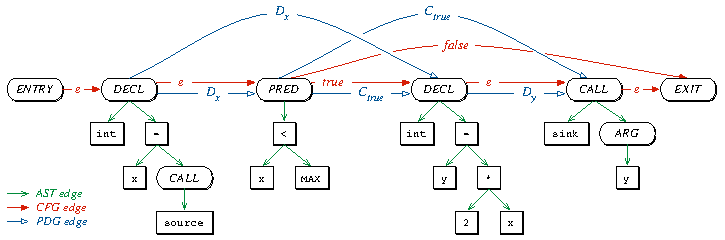
\includegraphics[width=0.98\textwidth]{figures/CPG.pdf}
	\caption{Code property graph for the code in Listing \ref{listing:cpg}. This figure was taken from~\cite{CPG-yamaguchi2014modeling}.}
	\label{figure:CPG}
\end{figure}

The CPG is then defined using the previous definitions of AST, CFG and PDG as: 

\begin{equation*}
    \mathcal{G} = ( \mathcal{V}_{\textsc{Ast}}, \mathcal{E}_{\textsc{Ast}} \cup \mathcal{E}_{\textsc{Cfg}} \cup \mathcal{E}_{\textsc{Pdg}}, \lambda, \mu )
\end{equation*}

\newpage
where the definition of the function $\lambda$ is as follows:

  \begin{equation*}
      \lambda(e) = 
      \begin{cases} 
      \lambda_{\textsc{Ast}} (e) \;\; \textit{if} \;\; e \in \mathcal{E}_{\textsc{Ast}} \\
      \lambda_{\textsc{Cfg}} (e) \;\; \textit{if} \;\; e \in \mathcal{E}_{\textsc{Cfg}} \\
      \lambda_{\textsc{Pdg}} (e) \;\; \textit{if} \;\; e \in \mathcal{E}_{\textsc{Pdg}} 
   \end{cases}
  \end{equation*}

and the definition of $\mu$ function is:
  
  \begin{equation*}
      \mu(x, p) = 
      \begin{cases} 
      \mu_{\textsc{Ast}} (x, p) \;\; \textit{if} \;\; (x, p) \in \mathcal{V}_{\textsc{Ast}} \bigtimes K_{\textsc{Ast}} \\
      \mu_{\textsc{Pdg}} (x, p) \;\; \textit{if} \;\; (x, p) \in \mathcal{E}_{\textsc{Pdg}} \bigtimes K_{\textsc{Pdg}} \\
   \end{cases}
  \end{equation*}

\iffalse
\begin{multicols}{2}
  \begin{equation*}
      \lambda(e) = 
      \begin{cases} 
      \lambda_{\textsc{Ast}} (e) \;\; \textit{if} \;\; e \in \mathcal{E}_{\textsc{Ast}} \\
      \lambda_{\textsc{Cfg}} (e) \;\; \textit{if} \;\; e \in \mathcal{E}_{\textsc{Cfg}} \\
      \lambda_{\textsc{Pdg}} (e) \;\; \textit{if} \;\; e \in \mathcal{E}_{\textsc{Pdg}} 
   \end{cases}
  \end{equation*}\break
  \begin{equation*}
      \mu(x, p) = 
      \begin{cases} 
      \mu_{\textsc{Ast}} (x, p) \;\; \textit{if} \;\; (x, p) \in \mathcal{V}_{\textsc{Ast}} \bigtimes K_{\textsc{Ast}} \\
      \mu_{\textsc{Pdg}} (x, p) \;\; \textit{if} \;\; (x, p) \in \mathcal{E}_{\textsc{Pdg}} \bigtimes K_{\textsc{Pdg}} \\
   \end{cases}
  \end{equation*}
\end{multicols}
\fi

A CPG for the code in Listing \ref{listing:cpg} is shown in Figure \ref{figure:CPG}.

\section{LLVM-Slicer}
\label{slicer}

LLVM-slicer is an open-source\footnote{\textbf{LLVM-Slicer}' repository: \url{https://github.com/mchalupa/dg}.} tool using DG library \cite{DG-2-chalupa2020dg, DG-chalupa2020dg}. The DG library implements various interprocedural static analyses namely \textit{pointer analysis}, d\textit{ata dependence analysis}, \textit{control dependence analysis} and \textit{value relationship analysis}. These analyses are implemented in DG as independent of the input language. However, the front-end currently supports only LLVM bitcode \cite{LLVM-bitcode}. LLVM bitcode is a \textit{storage format} for LLVM IR\footnote{\textbf{LLVM intermediate representation (LLVM IR)}.} \cite{LLVM-IR}, which is an \textit{assembly language} used as a low-level representation of code during the various stages of LLVM compilation.

The main use of the DG library is the aforementioned LLVM-slicer, which uses DG analysis for program-slicing - removing pieces of code that have no effect on \textit{user-defined} areas in the code. Experiments and results of slicing success on benchmarks from the Software Verification Competition can be found in \cite{DG-chalupa2020dg}. Although LLVM bitcode is language-independent and can be generated from e.g. C, C++, or Rust, LLVM-slicer does not support certain constructs in LLVM bitcode that handle \textit{exceptions}. This means that it is not able to handle a C++ program that uses exceptions. If the C++ code is exception-free, it should be able to slice it. The input to the LLVM-slicer is a single LLVM bitcode file and the output is the sliced LLVM bitcode.

\section{LLVM2CPG}
\label{llvm2cpg}

LLVM2CPG is an open-source\footnote{\textbf{LLVM2CPG}'s repository: \url{https://github.com/ShiftLeftSecurity/llvm2cpg}.} tool for constructing CPGs (defined in Section \ref{cpg}) from LLVM bitcode. The original CPG was created for high-level languages such as C, which creates some problems when creating CPGs from low-level LLVM IR \cite{llvm2cpg-webpage}. One problem is mapping LLVM IR instructions to classical high-level operations in order to display the CPG in the same format as e.g. the original C source code. Some operations can be mapped directly because they have the same \textit{semantics}, others can be modeled using functions, and some cannot be mapped at all and need to be bypassed by another mechanism. The CPG output format can be further processed by Ocular\footnote{\textbf{Ocular}'s documentation: \url{https://docs.shiftleft.io/ocular/quickstart}.} (proprietary), Plume\footnote{\textbf{Plume}'s documentation: \url{https://plume-oss.github.io/plume-docs/}.} (open-source) or Joern (open-source, see Section \ref{joern}).


\section{Joern}
\label{joern}

Joern \cite{joern-website} is a very powerful open-source\footnote{\textbf{Joern}'s repository: \url{https://github.com/joernio/joern}.} platform providing various tools in the area of static analysis. Using Joern, it is possible to write custom static analyses or \textit{queries} over source files. Joern supports the \textit{programming languages} C, C++, JavaScript, Kotlin, Python and Java. It is also possible to analyze Java bytecode or binary programs for the x86 architecture. It is also possible to construct different graph representations of the code (ASTs, CFGs, CDGs, DDGs, PDGs or CPGs), which can be exported in different formats e.g. DOT \cite{DOT} or \textbf{csv for the Neo4j graph database} \cite{neo4j-webpage}. It is also possible to load already constructed CPGs in different formats e.g. in the output format of the LLVM2CPG tool. Joern can be used as a \textit{command line} tool, through an \textit{interactive environment} or as an \textit{integration library}. Although Joern is a very diverse tool, it is only used in this term project as a format \textit{transformer} and is therefore described here very briefly.


\chapter{Constructing Graphs from Source Code}
\label{pipeline}

This chapter describes the design of a pipeline for constructing code property graphs from real-world C programs. Specifically, the introduction of this chapter describes the disadvantages of current approaches, the motivation for creating this pipeline, and its general principle. Section \ref{capture-phase} describes the principle of connecting the pipeline to the build process and preprocessing the inputs of the graph construction phase. Section \ref{construction-phase} describes the principle of constructing graphs from LLVM bitcode and Meta Infer outputs.

\begin{figure}[hbt]
	\centering
	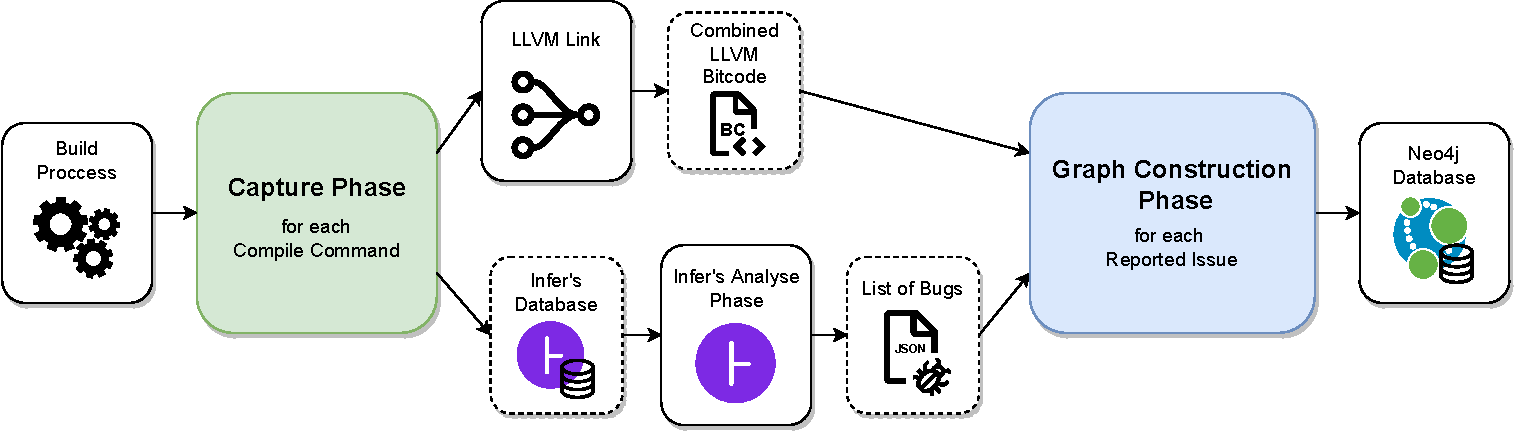
\includegraphics[width=0.99\textwidth]{figures/all.drawio.pdf}
	\caption{A simplified block diagram of a complete pipeline for constructing code property graphs from C source files. The dashed line indicates intermediate products. The diagram uses icon from \cite{infer-web}.}
	\label{figure:pipeline-all}
\end{figure}

When using a GNN to find vulnerabilities in programs, it is first necessary to convert the source code of the program into a suitable graph representation. The information in Section~\ref{cpg} shows that a suitable and frequently used representation is CPG. Each application of GNN to source code is preceded by some mechanism for constructing the type of graph used. However, the currently used graph construction approaches have a~number of disadvantages, which inspired the creation of this pipeline. The three main disadvantages of existing solutions are:

\begin{enumerate}
    \item construction of insufficient graph representation, e.g. construction of only AST \cite{GNN5-vsikic2022graph}, XFG \cite{GNN3-cheng2021deepwukong} or CFG \cite{GNN7-RNN-rabheru2020hybrid} (however, this paper uses a hybrid approach of GNN and RNN),
    \item not considering \textit{conditional compilation} \cite{GNN1-cao2021bgnn4vd, JOERN-CPG-guan2020code, GNN4-IBM-suneja2020learning, JOERN-CPG-xiaomeng2018cpgva, GNN2-zhou2019devign},
    \item inability to automatically construct graphs for arbitrary software \cite{GNN1-cao2021bgnn4vd, JOERN-CPG-guan2020code, GNN4-IBM-suneja2020learning, JOERN-CPG-xiaomeng2018cpgva, GNN2-zhou2019devign}.
\end{enumerate}

The last two points are closely linked. The previous works, namely \cite{GNN1-cao2021bgnn4vd, JOERN-CPG-guan2020code, GNN4-IBM-suneja2020learning, JOERN-CPG-xiaomeng2018cpgva, GNN2-zhou2019devign} all use the Joern tool (see Section \ref{joern}) to construct the CPG (and its various modifications), so they are also mentioned in both 2) and 3). Although Joern is a very useful tool, its disadvantage is that it analyses the source files directly and is not able to connect to the build process itself. This makes it unable to identify which source files to process and which not to. While Joern can \textit{recursively} find and process source files in a given directory \cite{joern-doc}, it does indeed process everything it finds in those directories. This becomes a problem if the software includes different versions of the source code, e.g. for different \textit{operating systems} (Windows or Linux), which are selected only during compilation. Joern will thus not be able to correctly construct a CPG without knowing which file to use in a given context. Therefore, Joern cannot be fully automatically deployed on arbitrary software. 

There is a similar problem with conditional compilation, where Joern cannot know which part of the code to use, or what values the macros (which are defined only during compilation) have. In experiments, it was found that Joern assumes that all macros are undefined by default, and thus irretrievably loses pieces of code that did not pass \texttt{\#ifdef} or \texttt{\#ifndef} conditions during preprocessing. These problems do not seem to manifest themselves in artificial datasets, and for concrete real-world software, these problems must be solved manually if using pure Joern.

The use case of the proposed pipeline is also subtly different from previous works. Here we need to construct graphs from the code with respect to the Infer report that has to be verified. However, this only requires the ability to slice the code according to the extracted information from the report. The program-slicing is also used in previous works. Thus, in this respect, the previous works differ only in the way the \textit{slicing properties} are specified and extracted.

The proposed pipeline is designed to construct CPGs from software written in C and a~subset of C++. The limitation for C++ is caused by the use of LLVM Slicer, the specific reasons are discussed more in Section \ref{slicer}. A simplified \textit{block diagram} of the complete pipeline is shown in Figure \ref{figure:pipeline-all}. The pipeline can be divided into two main parts:
 
\begin{enumerate}
    \item Capture Phase - the goal of this part is to connect to the running build process and extract the information needed to build the graphs.
    \item Graph Construction Phase - from the captured information in the capture phase, a~CPG graph is constructed and stored for each vulnerability found by Infer.
\end{enumerate}

The output of the whole process is a set of graphs, one graph for each vulnerability found by Infer. The output graphs are sliced to contain only information useful for future classification. Graphs simplified in this way will facilitate model learning. The graphs are stored in the Neo4j graph database, which then allows the data to be further processed, displayed, edited or passed to the GNN model.


\section{Capture Phase}
\label{capture-phase}

\begin{figure}[hbt]
	\centering
	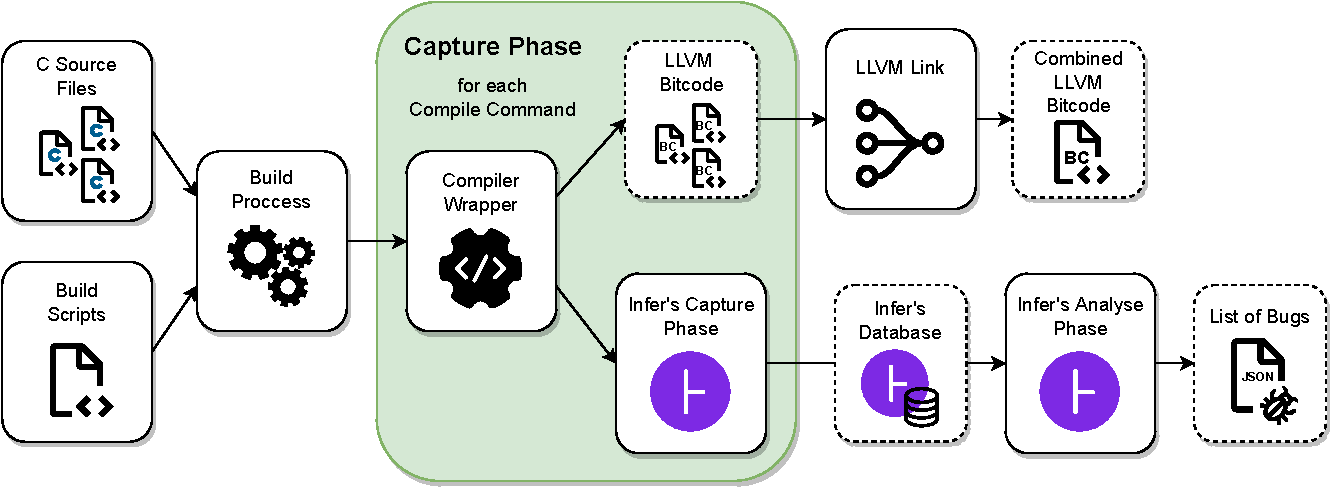
\includegraphics[width=0.99\textwidth]{figures/capture.drawio.pdf}
	\caption{A block diagram of the capture phase of the pipeline for extracting code property graphs from C source files. The dashed line indicates intermediate products. The diagram uses icons from \cite{infer-web, icon-compiler}.}
	\label{figure:pipeline-capture}
\end{figure}

The goal of the capture phase is to connect to the running build process and capture from it the information needed for the graph construction phase (see Section  \ref{figure:pipeline-capture}). This needed information is the source files transformed into LLVM bitcode and the same source files captured by the capture phase of Infer (see Section \ref{infer}). However, in order to obtain this information, it is necessary to obtain compilation commands from the build process. This can be done in two ways:

\begin{enumerate}
    \item by \textit{parsing} build scripts,
    \item by capturing with the \textit{compiler wrapper}.
\end{enumerate}

Parsing build scripts is very challenging because each build system uses different \textit{syntax} and techniques. However, there are build systems that have built-in extraction of compilation commands, such as cmake \cite{cmake-doc}. Unfortunately, this feature is far from being present in all build systems. Another problem is that there are software that do not use any of the standard build systems. Instead, they use custom scripts for compilation, \textit{linking}, etc. These scripts can of course have any structure and \textit{hierarchy of calls} to other scripts or tools, so it is almost impossible to statically parse compilation commands from them. The use of such scripts is quite common in SRPM packages (tool source packages for Fedora and CentOS) as seen in \cite{bc}. This pipeline is intended for use on SRPM packages and thus has to take this feature into account, see more in Section \ref{csmock}. For the reasons mentioned above, it follows that parsing build scripts, for previously unknown software, is generally not suitable for practical use.

The second and practically usable option is to create wrappers over C/C++ (or any other if needed) compilers and catch compilation commands at run-time. The design and implementation was covered in the author's previous work \cite{bc}, so the principle of wrappers will only be briefly described here. Each time a compiler is called by the build system, the installed wrapper is called. On each such call, the wrapper captures its \textit{arguments} and performs the following steps:

\begin{enumerate}
    \item filters out options that are not compatible with Infer's internal clang compiler, which Infer uses to transform source files into SIL (see Section \ref{infer}),
    \item calls the Infer's capture phase and passes the modified compilation command to it, Infer then saves the captured source files in SIL representation to its database,
    \item calls the original, unchanged, command so that the build can finish without problems.
\end{enumerate}

The wrapper is designed so that even if the capture phase of the Infer fails, the original command is still executed. Failure of the Infer's capture phase will not cause the entire analysis/pipeline to crash, it may just increase the chance of generating a false positive. This error recovery is possible due to the features of Infer, which, when it does not have the necessary implementations of the functions being analyzed captured, reason that they can return any value (limited by their return type, of course). This speculation introduces a degree of \textit{over-approximation} and thus introduces false positives. An important note is that these compiler wrappers can be (and typically are) called in \textit{parallel}. Thus, care must be taken with possible \textit{critical sections} such as the Infer database. Again, a description of how critical sections are handled in the wrapper can be found in \cite{bc}.

For this pipeline, it is necessary to add additional wrapper functionality - generating LLVM bitcode from each captured compilation command. LLVM bitcode can be generated using the clang compiler, by inserting certain options into each captured command that does the compilation (not linking, \textit{preprocessing} nor other things). It is needed to insert the following options in the order listed:
\begin{enumerate}
    \item \texttt{-emit-llvm} -- ensures that LLVM bitcode is generated instead of \textit{object}/\textit{binary files},
    \item \texttt{-g} -- allows \textit{backward mapping} of LLVM bitcode to the original source code,
    \item \texttt{-grecord-command-line} -- inserts debug information into the LLVM bitcode \cite{clang-doc},
    \item \texttt{-fno-inline-functions} -- disables the use of \textit{inline functions},
    \item \texttt{-fno-builtin} -- disables inserting compiler \textit{builtin functions}.
\end{enumerate}

It is also necessary to remove the \texttt{-o} option and its value so that LLVM bitcode files are generated instead of original output. The last thing the wrapper must do is find all LLVM bitcode files on the system when it is first called after initialization. A list of these files is stored and used after the capture phase to determine which LLVM bitcode files were recently created and thus belong to the build that just finished.

After the build (capture phase of the pipeline) is complete and before the graph construction phase is started, there are three more steps to take. First, find all LLVM bitcode files that were created during the capture phase. Simply create a list of all LLVM bitcode files currently present on the system and remove any that were present before the first compilation command was executed (the previously mentioned list created at the beginning of the capture phase is useful for this). Second, merge these newly created files into a~single one using the open-source\footnote{\textbf{llvm-link}'s repository: \url{https://github.com/llvm-mirror/llvm/tree/master/tools/llvm-link}.} tool llvm-link \cite{llvm-link-doc}. This step is here purely for practical purposes, see Section \ref{slicer}. And the last step is to run the Infer analysis (see Section \ref{infer}) on the captured files. After the analysis is complete, Infer will generate a list of found potential vulnerabilities.

The llvm-link tool, despite its name, has nothing to do with linking as used in compilers. It is purely about linking multiple files into a single one while preserving the LLVM bitcode format. This tool was chosen because of recommendations in the DG tool documentation, see section \ref{slicer}. Also, no alternative was found and it is an official tool provided by LLVM.

\section{Graph Construction Phase}
\label{construction-phase}

\begin{figure}[hbt]
	\centering
	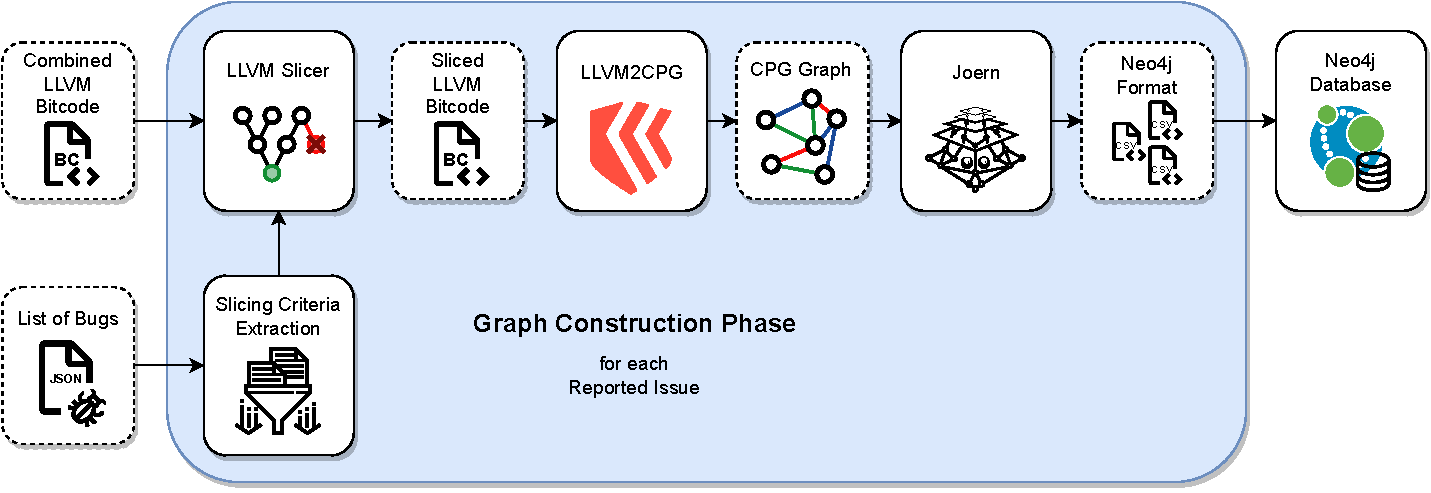
\includegraphics[width=0.99\textwidth]{figures/construction.drawio.pdf}
	\caption{A block diagram of the graph construction phase of the pipeline for extracting code property graphs from C source files. The dashed line indicates intermediate products. The diagram uses icons from \cite{joern-website, icon-funnel, icon-shiftleft}.}
	\label{figure:pipeline-construction}
\end{figure}

The input to the graph construction phase is two files (see Figure \ref{figure:pipeline-construction}), namely a file containing all the combined LLVM bitcode and a file with a list of the vulnerabilities found by Infer. The output of this phase is a single CPG for each vulnerability. The resulting CPGs are stored in the local Neo4j graph database.

\begin{lstlisting}[
    style=infer-format, label={listing:null-dereference}, float=hbt,
    caption={Null-dereference Infer report sample on the \texttt{coreutils} project.}
]
{
    "bug_type": "NULL_DEREFERENCE",
    "qualifier": "pointer `<@\textcolor{red}{new\_chunk}@>` last assigned on line 200 could be null and is dereferenced at line 204, column 3.",
    "severity": "ERROR",
    "line": <@\textcolor{greencomments}{204}@>,
    "column": 3,
    "procedure": "<@\textcolor{blue}{\_obstack\_newchunk}@>",
    "procedure_start_line": 181,
    "file": "lib/obstack.c",
    "bug_trace": [
        ...
    ],
    ...
}
\end{lstlisting}

\begin{lstlisting}[
    style=infer-format, label={listing:uninit}, float=hbt,
    caption={Uninitialized value Infer report sample on the \texttt{coreutils} project.}
]
{
    "bug_type": "UNINITIALIZED_VALUE",
    "qualifier": "The value read from <@\textcolor{red}{n\_read}@> was never initialized.",
    "severity": "ERROR",
    "line": <@\textcolor{greencomments}{412}@>,
    "column": 15,
    "procedure": "<@\textcolor{blue}{elide\_tail\_bytes\_pipe}@>",
    "procedure_start_line": 247,
    "file": "src/head.c",
    "bug_trace": [
        ...
    ],
    ...
}
\end{lstlisting}

First, the information needed for the program-slicing must be extracted from each Infer report. This information includes the \textit{entry point function} (where the program-slicing should start from), the variable/variables and their rows by which the combined LLVM bitcode will be sliced. The problem with slicing criteria extraction is that it has to be adjusted for a specific static analyzer output format (in this case for Infer). In addition, the Infer output format also varies subtly for different reported vulnerability types. Consider now two reports from Infer reported on the open-source\footnote{\textbf{coreutils}'s repository: \url{https://github.com/coreutils/coreutils}.} project \texttt{coreutils} -- null-dereference and uninitialized value, shown in Listing \ref{listing:null-dereference} and Listing \ref{listing:uninit} respectively. From both reports we need to get color-coded information. The function entry point (blue) and the variable usage line (green) can be extracted from both cases (and from all other vulnerability types) in the same way. However, the variable (red) to be sliced by is only listed as part of the vulnerability-specific description. For other bug types, the way of extracting the slicing criteria can be even more different, e.g. for buffer-overrun this information has to be extracted from the \texttt{bug\_trace} entry. This implies that it will be necessary to examine all Infer bug types and manually create slicing criteria extraction for each of them. An important note is that to use a different static analyzer, only the slicing criteria extraction needs to be adjusted (and of course the static analyzer needs to be run, but this is not a problem thanks to csmock, see Section \ref{csmock}).


\iffalse %%%%%%%%%%%%%%%%%%%%%%%%%%%%%%%%%%%%%%%%%%%%%%%%%%%%%%%%%%%%%%%%%%%%%%%%%%%%%
    {
        "bug_type": "NULL_DEREFERENCE",
        "qualifier": "pointer `new_chunk` last assigned on line 200 could be null and is dereferenced at line 204, column 3.",
        "severity": "ERROR",
        "line": 204,
        "column": 3,
        "procedure": "_obstack_newchunk",
        "procedure_start_line": 181,
        "file": "lib/obstack.c",
        "bug_trace": [
            ...
        ],
        "key": "obstack.c|_obstack_newchunk|NULL_DEREFERENCE",
        "node_key": "31bb46e2beb88c71793a7bb7e4d19eaf",
        "hash": "cf80c87901b71732a4b32feeefff7a82",
        "bug_type_hum": "Null Dereference"
    },

    {
        "bug_type": "BUFFER_OVERRUN_L1",
        "qualifier": "Offset: [2, +oo] Size: 2 by call to `quotearg_n_style`.",
        "severity": "ERROR",
        "line": 257,
        "column": 7,
        "procedure": "process_file",
        "procedure_start_line": 187,
        "file": "src/chmod.c",
        "bug_trace": [
                ...
            {
                "level": 3,
                "filename": "gnulib/lib/quotearg.c",
                "line_number": 255,
                "column_number": 1,
                "description": "Parameter `*arg`"
            },
            {
                "level": 3,
                "filename": "gnulib/lib/quotearg.c",
                "line_number": 464,
                "column_number": 25,
                "description": "Array access: Offset: [2, +oo] Size: 2 by call to `quotearg_n_style` "
            }
        ],
        "key": "chmod.c|process_file|BUFFER_OVERRUN_L1",
        "hash": "53afba1df9d4bb15bef10c46acff7484",
        "bug_type_hum": "Buffer Overrun L1"
    },


        {
        "bug_type": "UNINITIALIZED_VALUE",
        "qualifier": "The value read from n_read was never initialized.",
        "severity": "ERROR",
        "line": 412,
        "column": 15,
        "procedure": "elide_tail_bytes_pipe",
        "procedure_start_line": 247,
        "file": "src/head.c",
        "bug_trace": [
            {
                "level": 0,
                "filename": "src/head.c",
                "line_number": 412,
                "column_number": 15,
                "description": ""
            }
        ],
        "key": "head.c|elide_tail_bytes_pipe|UNINITIALIZED_VALUE",
        "hash": "9a46479ddd4516d2cb2bb85d0254b686",
        "bug_type_hum": "Uninitialized Value"
    },
\fi

After extracting the information for program-slicing, the LLVM slicer (described in Section~\ref{slicer}) is called with the necessary parameters on the combined LLVM bitcode file (the same LLVM bitcode file is used for all vulnerabilities). The output is sliced LLVM bitcode. This is passed to the LLVM2CPG tool (described in Section \ref{llvm2cpg}), which constructs the CPG. One possible tool that can process the format from LLVM2CPG is Joern. Although Joern is a very powerful tool for various tasks in static analysis, it is only used in this pipeline as a transformer of the CPG format. In fact, Joern is able to transform CPG into \texttt{csv} format, which can be easily loaded into the Neo4j graph database. Thus, each CPG (for each vulnerability) is inserted into the Neo4j database in the last part of the pipeline. All possible node and edge properties of the resulting CPG are specified in the Joern documentation \cite{joern-doc}.

The LLVM slicer tool was selected on the recommendation of Ing. Viktor Malík. After verification, it was found that LLVM slicer meets all the requirements of the pipeline design. The tool is also under active development. An alternative to LLVM slicer is e.g. llvm-slicing\footnote{\textbf{llvm-slicing}'s repository: \url{https://github.com/zhangyz/llvm-slicing}.}, but this tool is no longer maintained for a long time. LLVM2CPG was chosen on the recommendation of the Joern tool documentation \cite{joern-doc}, which commonly uses LLVM2CPG and depends on it for its support of LLVM bitcode. The reason for choosing the Joern tool was that it is the main choice of most of the above mentioned articles that construct graphs for GNNs from source files. And the Neo4j database was chosen for several reasons. It is one of the most widely used graph databases and is very well \textit{optimized} for operations on stored graphs. Another reason is the intuitive documentation\footnote{\textbf{Neo4j database} documentation: \url{https://neo4j.com/docs/}.} and also the Python driver documentation\footnote{\textbf{Neo4j Python driver} documentation: \url{https://neo4j.com/developer/python/}.}, which will be useful for passing data into
GNN.


\chapter{Future Work}
\label{future-work}

This chapter describes the future work that, together with this term project, will constitute the Master's thesis. Section~\ref{automation} describes the automation of the proposed pipeline. Section~\ref{d2a} describes the selected dataset and its transformation to the required format. Section \ref{gnn-choice} describes the architecture requirements and briefly some existing architectures. Section \ref{self-training} briefly describes the self-training technique and its use in this thesis. Section~\ref{csmock} describes the planned integration with the csmock tool. Finally, Section \ref{experiments} describes the data that will be used to \textit{evaluate} the accuracy of the trained model.

\section{Automation of a Graph Construction}
\label{automation}

It is clear that the graph construction pipeline proposed in this term project must be fully automated in order to be usable. The goal of future thesis work is to detect false positives among the vulnerabilities reported by Infer on SRPM packages within the csmock tool (more in Section \ref{csmock}). Csmock is used to automatically analyze SRPM packages using various static analyzers. Infer has already been integrated into csmock, as previous work by the author \cite{bc}. Because of the integration into csmock, it is necessary that not only the pipeline, but also everything that follows it - graph preprocessing and classification using GNNs - is fully automated.

Automation is currently implemented for the capture phase, the input preprocessing
construction phase and the construction phase itself, except slicing criteria
extraction. This part turns out to be the most difficult part, as it requires individual
approach to different types of reported vulnerabilities.


\section{Construction of Graphs from D2A Dataset}
\label{d2a}

In order to create a graph neural network that detects false positives, it must first be trained for such a task. And for that, a suitable dataset is needed. D2A \cite{D2A-zheng2021d2a} is a~dataset created by researchers at IBM Research. The pipeline code to create it is open-source\footnote{\textbf{D2A}'s generation pipeline sources: \url{https://github.com/IBM/D2A}.}. It is a~dataset created from real-world open-source projects \cite{D2A-webpage} namely \texttt{ffmpeg}, \texttt{httpd}, \texttt{libav}, \texttt{libtiff}, \texttt{nginx} and \texttt{openssl}. D2A is created in a hybrid way combining \textit{manual labeling} and \textit{automatic generation}, see \cite{D2A-zheng2021d2a} for more details. This gives it interesting properties. Compared to manually generated datasets, it contains many more samples since it can be automatically generated. Unfortunately, however, it has lower \textit{accuracy}. In contrast to automatically generated datasets (synthetic), it has samples from real-world software.

The reason for using D2A in future work is that it was created using Infer and thus each sample contains detailed Infer output from which slicing criteria can be extracted. Furthermore, each sample contains information about the type of vulnerability (the types are given by Infer), its location, the correctness of the report and the bug trace. However, the samples do not contain graphs but the source code of all the functions that are listed in the Infer's bug trace of a particular vulnerability. For this reason, the source code will first need to be converted to CPGs. However, this transformation will be very resource expensive, as each sample needs to be compiled and run the pipeline proposed above over it.


\section{Graph Neural Network Architecture}
\label{gnn-choice}

The next step is to select and possibly implement a specific graph neural network architecture. An interesting note is that the eventual trained model will not depend on the programming language (due to the use of LLVM) or the static analyzer (since it is only used for extracting the slicing criteria). However, the architecture must satisfy a few requirements:
\begin{enumerate}
    \item must respect the CPG format (see section \ref{cpg}),
    \item be suitable for classification,
    \item not too large to train the model using D2A and self-training (see Section \ref{self-training}).
\end{enumerate}

Originally, the architecture chosen was from BGNN4VD \cite{GNN1-cao2021bgnn4vd}, which has a CCG as input, which is very similar to a CPG, except that it uses a DFG instead of a PDG. The goal was to detect whether a function is vulnerable or not (function-level vulnerability). However, the paper does not provide, neither a link to the model, nor detailed model specifications (number of layers, parameters, used activation functions, etc.). And unfortunately, it was not even possible to contact the authors of this article.

Another interesting architecture is Devign \cite{GNN2-zhou2019devign}. The model input is again a combination of AST, CFG, DFG and natural code sequence (NCS). NCS is just an added set of edges that explicitly states the order of tokens in the original code. The model is again designed for function-level classification. Other interesting models can be found, e.g. in papers \cite{GNN3-cheng2021deepwukong, GNN8-RNN-fang2022jstrong}.


\section{Self-training}
\label{self-training}
Self-training \cite{self-traning-webpage} is a relatively simple method that allows the use of \textit{unlabeled data} in arbitrary \textit{supervised learning} method. Thus, it is an extension of supervised learning that makes it \textit{semi-supervised}. In principle, it is an extension of the \textit{labeled dataset} with unlabeled samples as follows:

\begin{itemize}
    \item Train the model on the labeled dataset and then iteratively execute:
        \begin{enumerate}
            \item run the trained model on unlabeled data,
            \item add pseudo-labels to samples that have a high probability of correct \textit{prediction} (the model is very confident),
            \item create a dataset by combining \textit{labeled samples} and \textit{pseudo-labeled samples},
            \item train the model on the newly created dataset and jump to 1).
        \end{enumerate}
\end{itemize}

This technique ideally improves the \textit{generalization} and accuracy of the model. Vulnerability detection in particular is an ideal task for self-learning, as there is a relatively small amount of good quality labeled data available and on the other hand we have a large amount of unlabeled data. The unlabeled samples can be easily and quickly created using a designed pipeline that we run (without a model) within the csmock tool on SRPM packages.


\section{Integration with Csmock}
\label{csmock} 

As previously mentioned, this whole approach (graph construction pipeline and model) was designed for integration with the csmock tool \cite{CsmockFLOCK, CsmockAVM} and subsequent analysis of SRPM packages. The open-source\footnote{\textbf{csmock}'s repository: \url{https://github.com/csutils/csmock}.} tool csmock is used to automatically run static analyses over SRPM packages (tool source packages for Fedora and CentOS operating systems). The csmock tool uses the mock tool to create an isolated and controlled environment in which a~SRPM package is compiled. Static analyses are also run in this created environment. The basic principle of csmock is illustrated in Figure \ref{figure:csmock}. The Meta Infer tool has already been integrated into csmock as part of the author's Bachelor's thesis~\cite{bc}. 

\begin{figure}[hbt]
	\centering
	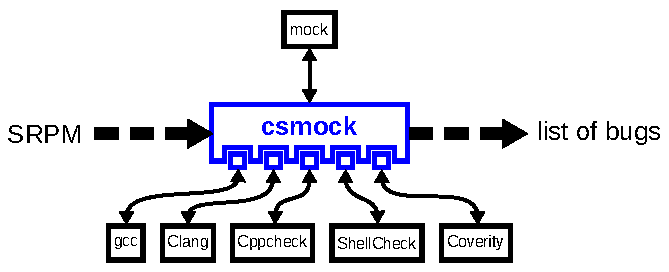
\includegraphics[width=0.9\textwidth]{figures/csmock.pdf}
	\caption{An illustration of the basic usage of the csmock tool for automated analysis of~SRPM packages. The figure was taken from \cite{CsmockAVM}.}
	\label{figure:csmock}
\end{figure}

Integrating this work into csmock will allow automatic checking of Infer reports. Since the model will produce a soft score for each error that indicates its probability of a false positive, the check can be approached in two ways. Either a hard decision will be made using the threshold and reports that have a high probability of being false positives will be filtered out. Or a soft score will be used to sort the reports. The idea behind this method is that no report that is potentially a true positive will be discarded, but if there is no time to check everything (which in practice there almost never is) it is possible to focus first on reports with a higher probability of being true positives according to the model. So ideally it should be possible to find most of the true positives in a first few of the reviewed reports.


\section{Experiments}
\label{experiments}

As mentioned earlier the output of this work should be applied to real-world software - SRPM packages. Ideally, experiments should be performed directly in this \textit{target domain}. The author's previous work \cite{bc} also include the analysis of several selected SRPM packages written in C using Infer. Specifically, these packages are \texttt{hostname}, \texttt{zip}, \texttt{cswrap}, \texttt{grep}, \texttt{make}, \texttt{mlocate}, \texttt{less}, \texttt{sed}, \texttt{tree} and \texttt{psmisc}. These analyses found a number of real bugs that were reported and fixed by the developers of the respective packages. The previous work makes it possible to evaluate the success of the model directly in the target domain and on real-world data with manual labels. There are approximately 400 manually labeled Infer reports on the above-mentioned SRPM packages and approximately another 200 on other software.

\chapter{Conclusion}
This term project first described static analysis in the context of finding vulnerabilities and the static analyzer Meta Infer. Then the basic concept of GNN was introduced, which served mainly as an introduction to the specification of GNN inputs. Then, one of the most widely used graph representations for finding vulnerabilities in source code -- code property graphs -- was introduced. This was followed by a description of the tools used. The core of the term project was a description of the design of a pipeline for automatic construction of code property graphs from source code. Finally, the thesis described the future steps needed to create a system for detecting false positives in Meta Infer reports.

The main contribution of this term project was the design of a pipeline for automatic extraction of code property graphs from source files written in C and a subset of C++. The goal of this design was to address the disadvantages of existing solutions, namely the disregard of conditional compilation and the inability to automatically identify source files to be analyzed. The proposed pipeline addresses both of these disadvantages thanks to its ability to connect to a running compilation process, from which all necessary information is extracted for the following construction of code property graphs. The pipeline also uses a~program slicing to remove unnecessary parts of the graphs in order to simplify the resulting graph and simplify future model training. The output CPGs are also independent of the input programming language of the pipeline due to the use of LLVM IR (as a source for constructing CPGs), however pipeline is still only applicable to C/C++. And since the Meta Infer report is only used as a source of slicing criteria, the output graphs are not dependent on a particular static analyzer either.

This term project will be followed by a Master's thesis that will focus on the design and development of a system for detecting false positives from the Meta Infer static analyzer. This system will consist of two parts. The first part is the pipeline proposed in this term project, which constructs code property graphs from the source code. The second part will be a trained graph neural network model that will classify the constructed graphs into false positives and true positives. This entire detection system is being designed with respect to integration into the csmock tool, so that the model can be used to inspect reports on SRPM packages.
